\chapter{Estabilidad del genoma: daño, reparación y recombinación del ADN}\label{ch:b3:dna-repair}

Una tarde en la playa introduce unas cien mil lesiones químicas en el ADN
de cada célula de la piel expuesta al sol: timinas contiguas soldadas en
dímeros por la luz ultravioleta, bases oxidadas, hebras mordidas. Sin sol
alguno, el agua tibia de la célula arranca cada día unas diez mil purinas
de sus azúcares y convierte centenares de citosinas en uracilo. Y sin
embargo la tasa de mutación de una célula humana es de un cambio por cada
diez mil millones de pares de bases y división --- en un genoma de seis
mil millones, menos de una mutación nueva por división. La distancia
entre el daño que sufre un genoma y el daño que conserva la cierra la
reparación: una docena de sistemas enzimáticos que patrullan la doble
hélice, reconocen lo que no debería estar ahí, lo recortan y lo
reconstruyen a partir de la hebra intacta y, cuando las dos hebras están
rotas, las vuelven a unir o copian el trozo perdido de una hermana. Los
niños a los que les falta uno de estos sistemas --- que se queman al
primer roce del sol, o que desarrollan un cáncer de colon a los treinta
--- muestran lo que valen. Este capítulo trata del daño, de las vías de
reparación, de la maquinaria de recombinación que repara las peores
roturas y que la meiosis toma prestada, y de la decisión de la célula,
cuando la reparación falla, de dejar de dividirse o de morir.

\section{Qué le va mal al ADN}

\begin{definition}[Lesiones del ADN]\label{def:b3:dna-repair:lesions}
\index{lesión del ADN}\index{depurinación}\index{desaminación}\index{dímero de pirimidina}\index{rotura de doble hebra}\index{8-oxoguanina}
Una \emph{lesión} es cualquier alteración química del ADN que se aparte
de las cuatro bases normales correctamente apareadas sobre un esqueleto
íntegro. Las lesiones espontáneas nacen de la química del agua y del
oxígeno: la \emph{depurinación}, la hidrólisis del enlace entre una
purina y su azúcar, que deja un sitio abásico (unos $10^{4}$ por célula y
día); la \emph{desaminación}, que convierte la citosina en uracilo, la
5-metilcitosina en timina y la adenina en hipoxantina (unos cuantos
centenares al día); la \emph{oxidación} por especies reactivas de
oxígeno, sobre todo a \emph{8-oxoguanina}, que se aparea con la adenina
con la misma facilidad que con la citosina; y los \emph{errores de
replicación}, una base mal incorporada o deslizada. Entre las lesiones
ambientales están el \emph{dímero ciclobutánico de pirimidina} y el
fotoproducto 6-4 que la luz ultravioleta produce entre dos pirimidinas
contiguas; las bases alquiladas por agentes alquilantes (la
O$^{6}$-metilguanina se aparea con la timina); los aductos voluminosos de
los hidrocarburos aromáticos y de la aflatoxina; los entrecruzamientos
entre hebras del cisplatino y de las mostazas nitrogenadas; y las roturas
de una y de \emph{dos hebras} que produce la radiación ionizante, unas
\num{1000} de hebra sencilla y \numrange{30}{40} de doble hebra por
célula y gray.
\end{definition}

\begin{proposition}[La escalera de la fidelidad]\label{prop:b3:dna-repair:fidelity}
\index{fidelidad}\index{corrección de pruebas}\index{reparación de errores de apareamiento}
La replicación alcanza su tasa de error de unos $10^{-10}$ por par de
bases en tres pasos multiplicativos. La selección de base por la
polimerasa, por geometría y por puentes de hidrógeno, se equivoca una vez
de cada $10^{5}$; la \emph{\omterm{prop:b3:dna-repair:fidelity}{corrección de pruebas}} por la exonucleasa
3$'\to$5$'$ de la polimerasa, que escinde una base terminal mal apareada
antes de la elongación, elimina el \qty{99}{\%} de esos errores; y la
\emph{\omterm{prop:b3:dna-repair:fidelity}{reparación de errores de apareamiento}}, que actúa detrás de la
horquilla sobre la hebra recién fabricada, elimina el \qty{99.9}{\%} de
lo que queda. El producto
$10^{-5}\times 10^{-2}\times 10^{-3} = 10^{-10}$ es la tasa observada,
y un defecto en cualquiera de los dos
pasos correctores la sube cien o mil veces: esas células son
\emph{mutadoras}.
\end{proposition}

\begin{example}[Lesiones frente a mutaciones]\label{ex:b3:dna-repair:numbers}
Una célula humana de $6.4\times 10^{9}$ pares de bases que se divide una
vez al día acumula del orden de $10^{4}$--$10^{5}$ lesiones diarias y
unas $6.4\times 10^{9}\times 10^{-10} \approx 0.6$ mutaciones nuevas por
división: menos de una \omterm{def:b3:dna-repair:lesions}{lesión} de cada diez mil sobrevive para convertirse
en un cambio permanente. Las demás se reparan antes de que la replicación
las lea, y lo que la selección ha minimizado es la tasa de supervivencia
hasta la mutación, no la tasa de daño. La misma aritmética explica por
qué el número de mutaciones de un tumor o del esperma de un padre mayor
cuenta divisiones: las mutaciones que lleva una célula son, en primera
aproximación, las divisiones que ha sufrido por el error de cada
división.
\end{example}

\section{Reparación de una hebra dañada}

\begin{definition}[Reparación por escisión]\label{def:b3:dna-repair:excision}
\index{reparación por escisión de bases}\index{reparación por escisión de nucleótidos}\index{glicosilasa}\index{xerodermia pigmentosa}
La mayoría de las lesiones afectan a una sola hebra y se reparan
recortando el trozo dañado y copiando la otra hebra. La \emph{reparación
por escisión de bases} (BER) se ocupa de las lesiones pequeñas que no
deforman: una \emph{ADN-glicosilasa} específica de un tipo de base
errónea (la uracilo-ADN-glicosilasa, la glicosilasa de la 8-oxoG y varias
más) saca la base fuera de la hélice y la corta de su azúcar; una AP
endonucleasa muerde el esqueleto en el sitio abásico; una polimerasa
(Pol~$\beta$) retira el azúcar e inserta un nucleótido; y una ligasa
sella. La \emph{reparación por escisión de nucleótidos} (NER) se ocupa de
las lesiones voluminosas que deforman la hélice --- \omterm{def:b3:dna-repair:lesions}{dímeros de pirimidina},
aductos químicos --- sin reconocer la química de la \omterm{def:b3:dna-repair:lesions}{lesión} misma: se
detecta la deformación (por XPC, que rastrea el genoma, o por una
ARN-polimerasa detenida, en la rama acoplada a la transcripción), las
subunidades helicasas de TFIIH abren la hélice, se verifica el daño
(XPA), dos endonucleasas (XPF, XPG) cortan la hebra dañada a
\numrange{24}{32} nucleótidos de distancia, se libera el oligonucleótido,
y una polimerasa y una ligasa rellenan el hueco. La pérdida de cualquiera
de las siete proteínas XP causa la \emph{xerodermia pigmentosa}:
sensibilidad extrema al sol, pecas y una tasa de cáncer de piel mil veces
mayor.
\end{definition}

\begin{proof}[Evidencia]
Cleaver (1968) cultivó fibroblastos de piel de pacientes con \omterm{def:b3:dna-repair:excision}{xerodermia
pigmentosa}, los irradió con luz ultravioleta y les dio timidina
radiactiva fuera de la fase S. Las células normales incorporaron la
marca en muchos puntos pequeños --- la ``síntesis de ADN no programada''
de los parches de reparación ---, mientras que las de los pacientes no
incorporaron casi nada y morían a dosis que las normales sobrevivían: la
enfermedad es un fallo al escindir los dímeros. La fusión de células de
dos pacientes restauraba a menudo la reparación en el híbrido, cada
célula aportando lo que a la otra le faltaba; con esta prueba los
pacientes se ordenaron en grupos de complementación de la A a la G, uno
por gen de la vía, años antes de que se clonaran los genes.
\end{proof}

\begin{omfigure}
\begin{tikzpicture}[every node/.style={font=\scriptsize}, >=stealth]
  % BER column
  \node[font=\small\bfseries] at (2.0,3.2) {Reparación por escisión de bases};
  \foreach \y/\txt in {2.6/{base dañada (U, 8-oxoG)}, 1.5/{la glicosilasa retira la base}, 0.4/{la AP endonucleasa muerde}, -0.7/{la Pol $\beta$ rellena un nucleótido, la ligasa sella}} {
    \draw[very thick, omDef] (0.2,\y) -- (3.8,\y); \draw[very thick, omDef] (0.2,\y-0.25) -- (3.8,\y-0.25);
    \node[right, align=left] at (0.2,\y-0.6) {\txt};
  }
  \fill[omThm] (2.0,2.6) circle (0.1);
  \draw[omThm, thick] (1.9,1.5) -- (2.1,1.5);
  \draw[white, very thick] (1.9,0.4) -- (2.1,0.4);
  \fill[omMeth!80!black] (2.0,-0.7) circle (0.1);
  % NER column
  \node[font=\small\bfseries] at (8.0,3.2) {Reparación por escisión de nucleótidos};
  \foreach \y/\txt in {2.6/{una lesión voluminosa deforma la hélice; XPC se une}, 1.5/{TFIIH abre la hélice, XPA verifica}, 0.4/{XPF y XPG cortan a 24--32 nt}, -0.7/{la polimerasa rellena el hueco, la ligasa sella}} {
    \draw[very thick, omDef] (6.2,\y) -- (9.8,\y); \draw[very thick, omDef] (6.2,\y-0.25) -- (9.8,\y-0.25);
    \node[right, align=left] at (6.2,\y-0.6) {\txt};
  }
  \draw[omThm, very thick] (7.8,2.6) -- (8.2,2.6) -- (8.2,2.75) -- (7.8,2.75) -- cycle;
  \draw[omDef, very thick] (7.2,1.5) .. controls (7.6,1.85) and (8.4,1.85) .. (8.8,1.5); \draw[omThm, very thick] (7.85,1.72) -- (8.15,1.72);
  \draw[very thick, white] (7.0,0.4) -- (9.0,0.4); \draw[omThm, thick, ->] (7.0,0.7) -- (7.0,0.48); \draw[omThm, thick, ->] (9.0,0.7) -- (9.0,0.48);
  \draw[very thick, omMeth!80!black] (7.0,-0.7) -- (9.0,-0.7);
\end{tikzpicture}

{\small Dos vías de escisión. La escisión de bases (izquierda) reconoce
una base errónea concreta con una \omterm{def:b3:dna-repair:excision}{glicosilasa} dedicada y sustituye un
solo nucleótido. La escisión de nucleótidos (derecha) reconoce la
deformación que causa cualquier \omterm{def:b3:dna-repair:lesions}{lesión} voluminosa, corta la hebra a ambos
lados y sustituye un parche de unos treinta nucleótidos (verde).}
\end{omfigure}

\begin{definition}[Reparación de errores de apareamiento]\label{def:b3:dna-repair:mmr}
\index{reparación de errores de apareamiento!discriminación de hebra}\index{síndrome de Lynch}\index{inestabilidad de microsatélites}
La \emph{\omterm{prop:b3:dna-repair:fidelity}{reparación de errores de apareamiento}} (MMR) corrige los malos
apareamientos y los pequeños bucles de inserción o deleción que escapan a
la \omterm{prop:b3:dna-repair:fidelity}{corrección de pruebas}. La proteína MutS (MSH2--MSH6 en el ser humano)
reconoce la deformación de un mal apareamiento y, con MutL (MLH1--PMS2),
autoriza a una exonucleasa a degradar la hebra recién sintetizada desde
una mordedura cercana hasta más allá del mal apareamiento; una polimerasa
rellena el hueco. La dificultad es la \emph{discriminación de hebra}: un
mal apareamiento tiene dos bases y solo una es la equivocada. En
\emph{Escherichia coli} la hebra nueva se identifica porque todavía no
está metilada en los sitios GATC, que la metilasa Dam marca unos minutos
después de la síntesis; MutH muerde la hebra no metilada. En los
eucariotas la hebra nueva se identifica por las mordeduras entre
fragmentos de Okazaki y por el extremo 3$'$ libre de la hebra
conductora. La pérdida de la MMR sube la tasa de mutación de cien a mil
veces, sobre todo y de manera visible en los \emph{microsatélites} ---
series de una repetición corta donde la polimerasa resbala ---, cuyas
longitudes cambian de una célula a otra: la \emph{inestabilidad de
microsatélites}. La pérdida heredada de un alelo de la MMR es el
\emph{síndrome de Lynch}, con cáncer colorrectal en cerca del
\qty{70}{\%} de los portadores, a menudo antes de los cincuenta.
\end{definition}

\begin{omfigure}
\begin{tikzpicture}[every node/.style={font=\scriptsize}, >=stealth]
  \draw[very thick, omDef] (0,1.2) -- (9,1.2); \node[left] at (-0.1,1.2) {hebra molde};
  \draw[very thick, gray] (0,0.6) -- (9,0.6); \node[left] at (-0.1,0.6) {hebra nueva};
  % methyl groups on template at GATC
  \foreach \x in {1.5,7.5} { \fill[omMeth!80!black] (\x,1.35) circle (0.1); \node[above] at (\x,1.45) {CH$_3$ en GATC}; }
  \foreach \x in {1.5,7.5} { \draw[omMeth!80!black] (\x,0.45) circle (0.1); }
  \node[below] at (7.5,0.32) {aún sin metilar};
  % mismatch
  \draw[omThm, very thick] (4.5,1.05) -- (4.5,0.75); \node[omThm, right] at (4.6,0.9) {mal apareamiento};
  \draw[thick, fill=omExo!35] (4.5,1.9) ellipse (1.0 and 0.3); \node at (4.5,1.9) {MutS/MutL};
  \draw[->, thick] (4.5,1.65) -- (4.5,1.3);
  % MutH nick on new strand at unmethylated GATC
  \draw[omThm, thick, ->] (1.5,-0.55) -- (1.5,0.42); \node[omThm, below] at (1.5,-0.55) {MutH muerde la hebra no metilada};
  % excision arrow
  \draw[->, very thick, omProp] (1.7,-0.1) -- (5.0,-0.1); \node[omProp, below] at (3.95,-0.15) {la exonucleasa degrada más allá del error};
  \node[right] at (5.4,-0.8) {luego la Pol III rellena el hueco y la ligasa sella};
\end{tikzpicture}

{\small La discriminación de hebra en la reparación bacteriana de errores
de apareamiento. La hebra molde lleva grupos metilo en sus sitios GATC;
la hebra nueva todavía no, y MutH la muerde ahí. La base equivocada se
quita por tanto siempre de la hebra nueva.}
\end{omfigure}

\begin{method}[Ordenar una enfermedad de reparación en genes]\label{met:b3:dna-repair:complementation}
\index{prueba de complementación}
Para averiguar cuántos genes intervienen en un fenotipo recesivo, antes
de conocer ninguno: (1) tómense líneas celulares de pacientes no
emparentados, cada una mutante en algún gen de la vía; (2) fusiónense
pares de líneas en células híbridas; (3) pruébese la función en el
híbrido (aquí, la síntesis de ADN no programada tras la luz
ultravioleta); (4) si el híbrido repara, los dos pacientes llevan
mutaciones en genes \emph{distintos} (cada uno aporta la proteína que al
otro le falta: se \emph{complementan}); si no, en el mismo gen; (5)
agrúpense los pacientes en grupos de complementación --- uno por gen. El
número de grupos es una cota inferior del número de genes.
\end{method}

\section{Reparación de un cromosoma roto}

\begin{definition}[Reparación de roturas de doble hebra]\label{def:b3:dna-repair:dsb}
\index{unión de extremos no homólogos}\index{recombinación homóloga}\index{Rad51}\index{unión de Holliday}\index{BRCA}
Una \emph{\omterm{def:b3:dna-repair:lesions}{rotura de doble hebra}} secciona el cromosoma y no deja ninguna
hebra intacta que copiar. Dos vías la reparan. La \emph{unión de extremos
no homólogos} (NHEJ): el anillo Ku70--Ku80 se une a cada extremo, recluta
a la quinasa DNA-PKcs, unas nucleasas recortan los salientes y la ligasa
IV une los extremos; funciona en cualquier fase del ciclo y en cuestión
de minutos, pero pierde o añade unos pocos nucleótidos en la unión y
puede unir los extremos equivocados. La \emph{recombinación homóloga}
(HR): el complejo MRN y unas nucleasas resecan las hebras 5$'$ para dejar
colas largas de hebra sencilla 3$'$, que recubre la RPA y después, con
ayuda de BRCA2, la recombinasa \emph{Rad51}; el filamento de Rad51 busca
un dúplex homólogo --- la cromátida hermana, en S y en G2 ---, lo invade,
y el extremo 3$'$ invasor ceba la síntesis sobre la copia intacta. Las
moléculas conjuntas pueden disolverse tras una síntesis corta (la mayor
parte de la reparación mitótica, sin intercambio del ADN flanqueante) o
madurar hasta dar dos \emph{uniones de Holliday} de cuatro brazos, cuya
resolución por endonucleasas da un producto con entrecruzamiento o sin
él. La HR es exacta porque copia a una hermana, pero solo está disponible
cuando existe una hermana.
\end{definition}

\begin{omfigure}
\begin{tikzpicture}[every node/.style={font=\scriptsize}, >=stealth]
  % break
  \draw[very thick, omDef] (0,3.2) -- (2.3,3.2); \draw[very thick, omDef] (2.7,3.2) -- (5,3.2);
  \draw[very thick, omDef] (0,3.0) -- (2.3,3.0); \draw[very thick, omDef] (2.7,3.0) -- (5,3.0);
  \node[above] at (2.5,3.3) {rotura de doble hebra};
  % NHEJ left
  \draw[->, thick] (1.2,2.8) -- (-0.5,2.0); \node[left, align=right] at (-0.6,2.4) {cualquier fase,\\minutos};
  \node[font=\small\bfseries] at (-1.6,1.55) {NHEJ};
  \draw[thick, fill=omExo!35] (-2.6,0.9) ellipse (0.3 and 0.2); \draw[thick, fill=omExo!35] (-0.8,0.9) ellipse (0.3 and 0.2);
  \draw[very thick, omDef] (-3.4,0.9) -- (-2.9,0.9); \draw[very thick, omDef] (-0.5,0.9) -- (0.0,0.9);
  \node[below] at (-1.7,0.7) {Ku une ambos extremos, recorte};
  \draw[->, thick] (-1.7,0.3) -- (-1.7,-0.1);
  \draw[very thick, omDef] (-3.4,-0.4) -- (0.0,-0.4); \draw[omThm, very thick] (-1.85,-0.4) -- (-1.55,-0.4);
  \node[below, align=center] at (-1.7,-0.55) {la ligasa IV une:\\se pierden o se añaden unos nucleótidos};
  % HR right
  \draw[->, thick] (3.8,2.8) -- (5.5,2.0); \node[right, align=left] at (5.6,2.4) {S/G2, con hermana\\presente; horas};
  \node[font=\small\bfseries] at (6.8,1.55) {HR};
  % resected ends
  \draw[very thick, omDef] (4.6,0.9) -- (6.2,0.9); \draw[very thick, omDef] (7.4,0.9) -- (9.0,0.9);
  \draw[very thick, omDef] (4.6,0.7) -- (5.6,0.7); \draw[very thick, omDef] (8.0,0.7) -- (9.0,0.7);
  \foreach \x in {5.7,5.9,6.1} \fill[omProp] (\x,0.9) circle (0.07);
  \node[below] at (6.8,0.55) {resección 5$'$; Rad51 recubre las colas 3$'$};
  \draw[->, thick] (6.8,0.15) -- (6.8,-0.25);
  % strand invasion of sister
  \draw[very thick, omMeth!70!black] (4.6,-0.9) -- (9.0,-0.9); \draw[very thick, omMeth!70!black] (4.6,-1.1) -- (9.0,-1.1);
  \draw[very thick, omDef] (4.6,-0.5) -- (5.8,-0.5) .. controls (6.2,-0.5) and (6.3,-0.9) .. (6.6,-0.9) -- (7.6,-0.9);
  \draw[->, omDef, thick] (7.6,-0.9) -- (8.1,-0.9);
  \node[below, align=center] at (6.8,-1.2) {invasión de la hermana (verde), síntesis sobre la copia intacta,\\luego disolución (sin entrecruzamiento) o uniones de Holliday};
\end{tikzpicture}

{\small Los dos destinos de una \omterm{def:b3:dna-repair:lesions}{rotura de doble hebra}. Izquierda: la
unión de extremos, rápida y siempre disponible, al precio de un pequeño
cambio en la juntura. Derecha: la \omterm{def:b3:dna-repair:dsb}{recombinación homóloga}, que reseca los
extremos, invade la cromátida hermana con un filamento de \omterm{def:b3:dna-repair:dsb}{Rad51} y copia
lo que se había perdido.}
\end{omfigure}

\begin{theorem}[Carga de daño, velocidad de reparación y la horquilla]\label{thm:b3:dna-repair:load}
\index{daño residual}\index{vías en competencia}
Supóngase que las lesiones de un tipo aparecen a velocidad constante $D$
por célula y hora y que las elimina una reparación de primer orden de
constante $k$ (semivida $t_{1/2} = \ln 2/k$). El número de lesiones
$L(t)$ obedece $\mathrm{d}L/\mathrm{d}t = D - kL$, de modo que en el
estado estacionario
\[
L^{*} = \frac{D}{k},
\]
y un pulso de $N$ lesiones administrado en $t = 0$ deja $N e^{-kT}$
lesiones cuando una horquilla de replicación llega en el instante $T$. Si
dos vías compiten por la misma \omterm{def:b3:dna-repair:lesions}{lesión} con constantes $k_{1}$ y $k_{2}$,
cada \omterm{def:b3:dna-repair:lesions}{lesión} la repara la primera con probabilidad $k_{1}/(k_{1} +
k_{2})$ y la semivida global es $\ln 2/(k_{1} + k_{2})$. El número de
lesiones que llegan a la horquilla sigue una distribución de Poisson de
media $N e^{-kT}$, de modo que la probabilidad de que no llegue ninguna
es $\exp(-N e^{-kT})$.
\end{theorem}
\begin{proof}
El estado estacionario es donde $D = kL$. Para el pulso, $D = 0$ y la
ecuación se integra hasta $L = N e^{-kt}$. Con dos vías la velocidad de
pérdida es $(k_{1} + k_{2})L$; en cualquier intervalo corto una \omterm{def:b3:dna-repair:lesions}{lesión}
dada la elimina la vía~1 con probabilidad $k_{1}\,\mathrm{d}t$ y la
vía~2 con $k_{2}\,\mathrm{d}t$, de modo que la probabilidad condicionada
de que su eliminación, cuando ocurra, sea por la vía~1 es $k_{1}/(k_{1} +
k_{2})$. Lesiones independientes que sobreviven cada una con probabilidad
$e^{-kT}$ dan un recuento binomial, de Poisson en el límite de muchas
lesiones y poca supervivencia, y la probabilidad de Poisson de cero es
$e^{-\text{media}}$.
\end{proof}

\begin{example}[Por qué la xerodermia es una enfermedad de la horquilla]\label{ex:b3:dna-repair:xp}
Una dosis de sol deja $N = 10^{5}$ \omterm{def:b3:dna-repair:lesions}{dímeros de pirimidina} en un
queratinocito. Con una semivida de escisión de nucleótidos de
\qty{2}{h} ($k =
\qty{0.35}{h^{-1}}$) y una horquilla a las \qty{8}{h}, quedan $N e^{-kT} =
10^{5}\times e^{-2.8} \approx 6000$ dímeros por copiar; con la
reparación casi ausente de una célula XP ($k \approx
\qty{0.01}{h^{-1}}$), son \num{92000}. Cada dímero que encuentra la
horquilla lo sortea la \omterm{def:b3:dna-repair:tls}{síntesis translesión} (más abajo), que es propensa
al error: la carga de mutaciones por división del paciente es quince
veces la normal, y los cánceres de piel llegan en la infancia. La cura
que funciona es mantener $N$ bajo --- la evitación total de la luz
ultravioleta.
\end{example}

\begin{omfigure}
\begin{tikzpicture}
\begin{axis}[
  width=0.7\linewidth, height=5.6cm,
  axis x line=bottom, axis y line=left,
  xmin=0, xmax=12, ymin=100, ymax=200000, ymode=log,
  xlabel={horas tras la exposición}, ylabel={dímeros por célula},
  xlabel style={font=\small, at={(axis description cs:0.5,-0.12)}, anchor=north},
  ylabel style={font=\small},
  tick label style={font=\small}, xtick={0,2,4,6,8,10,12},
  clip=false,
]
\addplot[very thick, omDef, domain=0:12, samples=40] {100000*exp(-0.35*x)};
\addplot[very thick, omThm, domain=0:12, samples=40] {100000*exp(-0.01*x)};
\addplot[dashed, gray] coordinates {(8,100) (8,200000)};
\node[font=\scriptsize, anchor=south east, gray] at (axis cs:8,110) {llega la horquilla};
\node[font=\scriptsize, omDef, anchor=north east] at (axis cs:11.5,18000) {normal, $t_{1/2} = \qty{2}{h}$};
\node[font=\scriptsize, omThm, anchor=south west] at (axis cs:2,105000) {xerodermia pigmentosa};
\fill[omDef] (axis cs:8,6070) circle (2pt); \node[font=\scriptsize, omDef, anchor=west] at (axis cs:8.3,6070) {\num{6000}};
\fill[omThm] (axis cs:8,92300) circle (2pt); \node[font=\scriptsize, omThm, anchor=north west] at (axis cs:8.3,80000) {\num{92000}};
\end{axis}
\end{tikzpicture}

{\small Dímeros que quedan tras un pulso de $10^{5}$, en escala
logarítmica, para una célula normal y otra deficiente en escisión de
nucleótidos. La horquilla, a las \qty{8}{h}, encuentra quince veces más
lesiones en la célula del paciente.}
\end{omfigure}

\begin{proof}[Evidencia]
Holliday (1964) propuso la unión de cuatro brazos para explicar un enigma
de la genética de los hongos: en un cruce, una tétrada de esporas
mostraba a veces una segregación $3{:}1$ en lugar de la mendeliana
$2{:}2$ de un marcador, siempre en marcadores próximos a un
entrecruzamiento. Su modelo --- el intercambio de hebras sencillas entre
dos dúplex homólogos, que forma un heterodúplex que la \omterm{prop:b3:dna-repair:fidelity}{reparación de
errores de apareamiento} ``corrige'' luego en un sentido o en el otro (la
\emph{conversión génica}) --- explicaba a la vez las proporciones
extrañas y su asociación con el entrecruzamiento. La unión misma se vio
después al microscopio electrónico en plásmidos en recombinación y en la
estructura de la resolvasa RuvC unida a ella.
\end{proof}

\section{Tolerancia, alarma y la decisión de parar}

\begin{definition}[Síntesis translesión]\label{def:b3:dna-repair:tls}
\index{síntesis translesión}\index{polimerasa eta}
Cuando una horquilla encuentra una \omterm{def:b3:dna-repair:lesions}{lesión} que no se ha reparado, la
polimerasa replicativa se detiene. La \emph{síntesis translesión} (TLS)
llama a una polimerasa especializada, de sitio activo más holgado y sin
\omterm{prop:b3:dna-repair:fidelity}{corrección de pruebas} --- la Pol~$\eta$ para los \omterm{def:b3:dna-repair:lesions}{dímeros de pirimidina}, y
las Pol~$\iota$, $\kappa$, $\zeta$ y Rev1 para otras lesiones ---, que
inserta unos pocos nucleótidos frente a la \omterm{def:b3:dna-repair:lesions}{lesión} y se aparta. La
Pol~$\eta$ pone dos adeninas frente a un dímero de timina, lo que suele
ser correcto; las demás se equivocan a menudo. La TLS cambia exactitud
por la supervivencia de la horquilla, y es la fuente de la mayoría de las
mutaciones inducidas por el ultravioleta. La forma variante de la
\omterm{def:b3:dna-repair:excision}{xerodermia pigmentosa} (XP-V) tiene intacta la reparación por escisión y
carece de Pol~$\eta$: los dímeros que escapan a la escisión los sortean
las polimerasas más propensas al error, y los cánceres llegan igual.
\end{definition}

\begin{proposition}[La respuesta SOS bacteriana]\label{prop:b3:dna-repair:sos}
\index{respuesta SOS}\index{RecA}\index{LexA}
En \emph{E.~coli} la recombinasa RecA, unida al ADN de hebra sencilla que
se acumula en las horquillas detenidas y en las roturas resecadas, se
convierte en una coproteasa que induce al represor LexA a cortarse a sí
mismo. LexA reprime unos cuarenta genes; a medida que cae, se van
encendiendo en orden de afinidad de sus operadores: primero los genes de
escisión \emph{uvrA} y \emph{uvrB}, luego el propio \emph{recA} y el
inhibidor de la división celular \emph{sulA} (las células dejan de
dividirse y crecen en filamentos), y por último las polimerasas propensas
al error Pol~IV y Pol~V, que sortean las lesiones a costa de mutaciones.
La respuesta graduada intenta primero la reparación exacta y solo recurre
a la tolerancia mutagénica cuando el daño persiste; las mutaciones que
induce son la materia prima sobre la que evoluciona la resistencia a los
antibióticos durante un tratamiento.
\end{proposition}

\begin{omfigure}
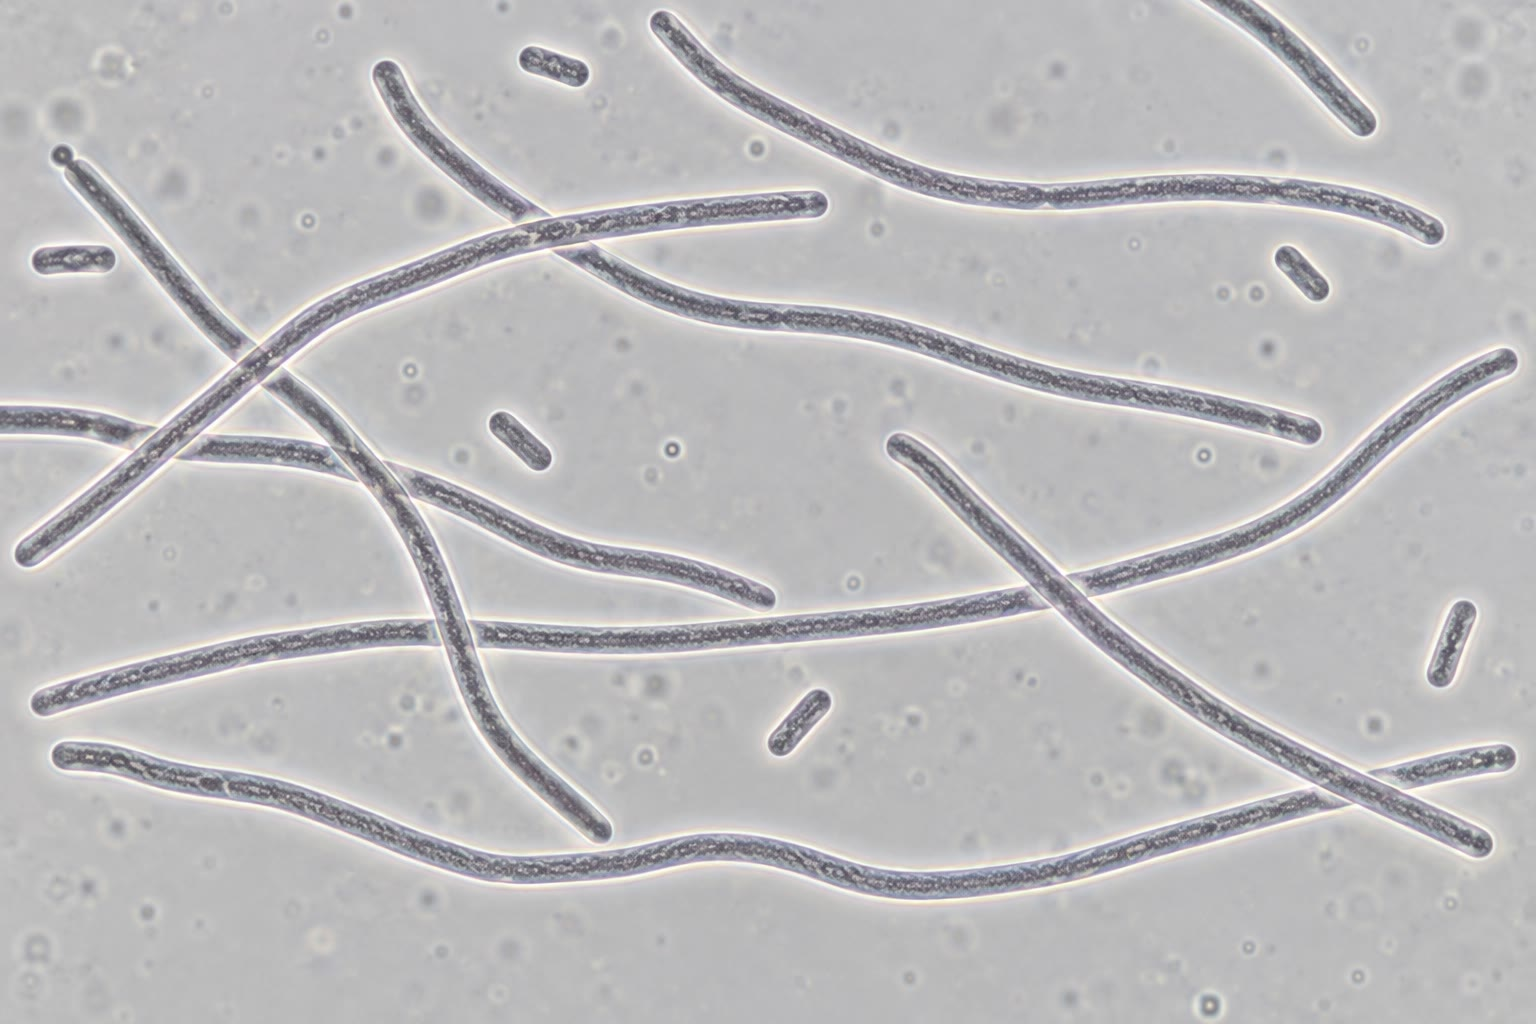
\includegraphics[width=0.46\linewidth]{images/book5/ai/b5-03-sos-filaments.jpg}\hspace{0.04\linewidth}
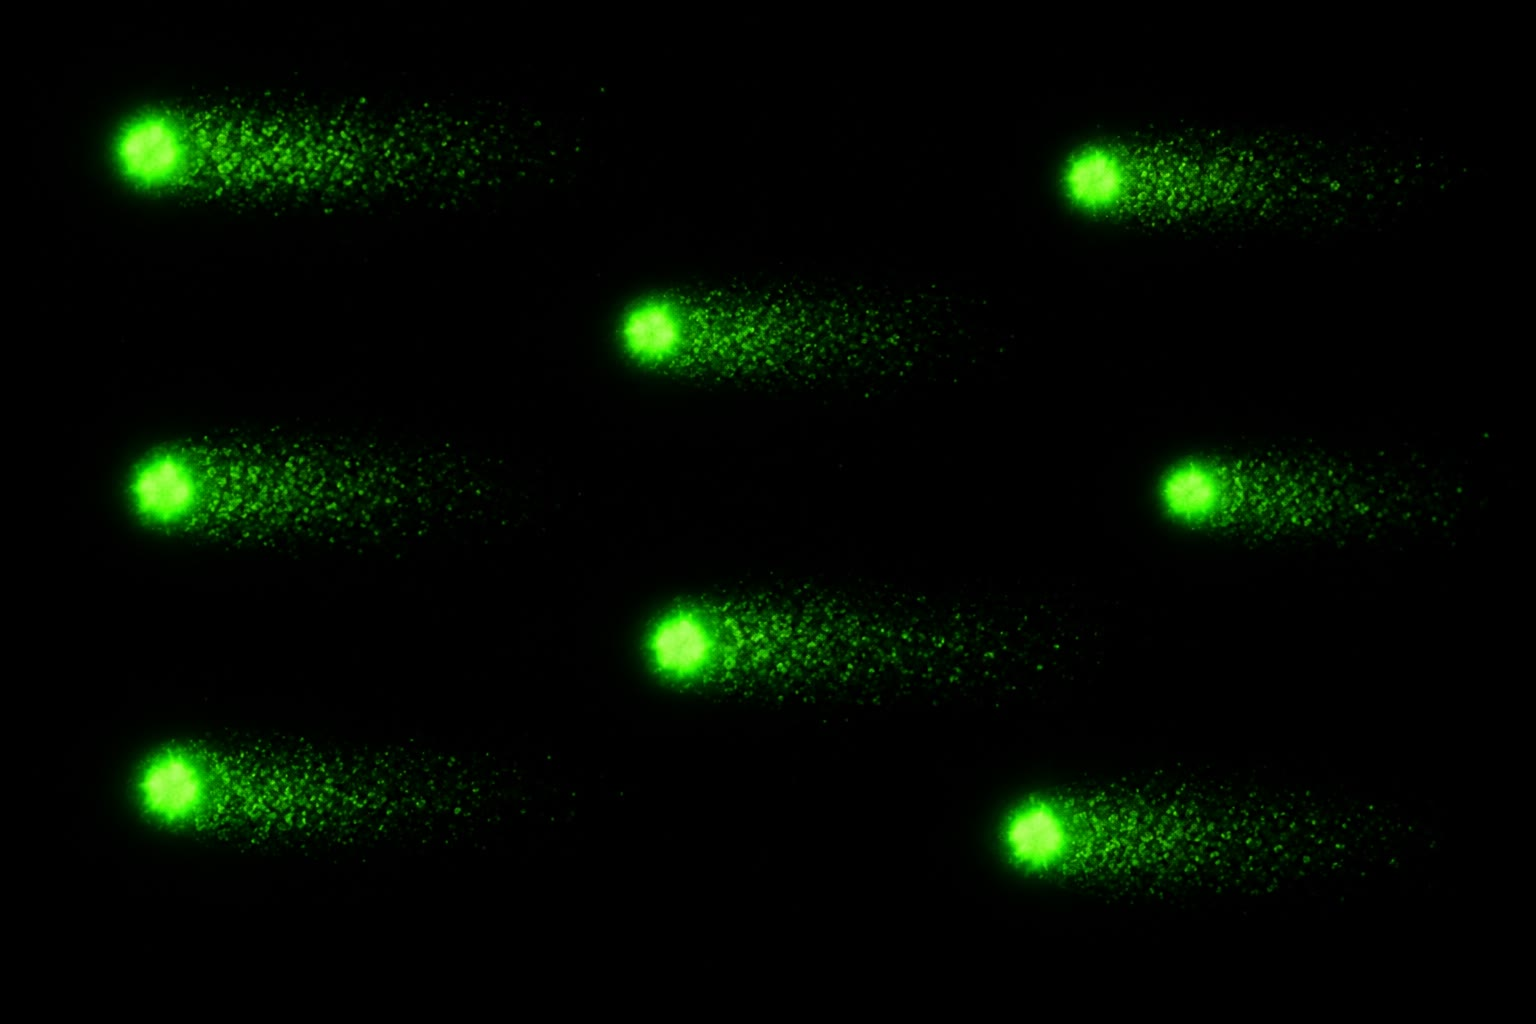
\includegraphics[width=0.46\linewidth]{images/book5/ai/b5-03-comet-assay.jpg}

{\small Izquierda: \emph{E.~coli} tras la irradiación ultravioleta,
crecida en filamentos largos porque la \omterm{prop:b3:dna-repair:sos}{respuesta SOS} ha bloqueado la
división celular mientras se repara el ADN. Derecha: un ensayo cometa ---
células sueltas embebidas en un gel y sometidas a electroforesis; el ADN
fragmentado sale del núcleo formando una cola cuya longitud mide el
número de roturas.}
\end{omfigure}

\begin{definition}[La respuesta al daño del ADN]\label{def:b3:dna-repair:ddr}
\index{respuesta al daño del ADN}\index{ATM}\index{punto de control}\index{p53}\index{gamma-H2AX}
Los eucariotas señalan el daño mediante dos quinasas: \emph{ATM}, que el
complejo MRN recluta a las \omterm{def:b3:dna-repair:lesions}{roturas de doble hebra}, y \emph{ATR}, que se
recluta al ADN de hebra sencilla de las horquillas detenidas. Fosforilan
centenares de dianas. En cuestión de minutos se fosforila la \omterm{def:b3:chromatin-epigenetics:nucleosome}{histona}
H2AX (\emph{$\gamma$-H2AX}) a lo largo de megabases alrededor de cada
rotura, lo que forma un foco que recluta proteínas de reparación y que
puede contarse al microscopio, un foco por rotura. Las quinasas Chk1 y
Chk2 detienen el ciclo celular --- los \emph{puntos de control} del
\cref{ch:b3:cell-cycle-apoptosis} --- inactivando las fosfatasas que
impulsarían la entrada en S o en M; y el factor de transcripción
\emph{p53}, estabilizado por fosforilación, induce el inhibidor de
quinasas dependientes de ciclina p21 (una parada duradera en G1), los
genes de reparación y, si el daño es grande o persiste, los genes
apoptóticos que matan a la célula. La respuesta compra tiempo para la
reparación y, cuando la reparación falla, elimina la célula en lugar de
dejarla dividirse con el genoma roto.
\end{definition}

\begin{omfigure}
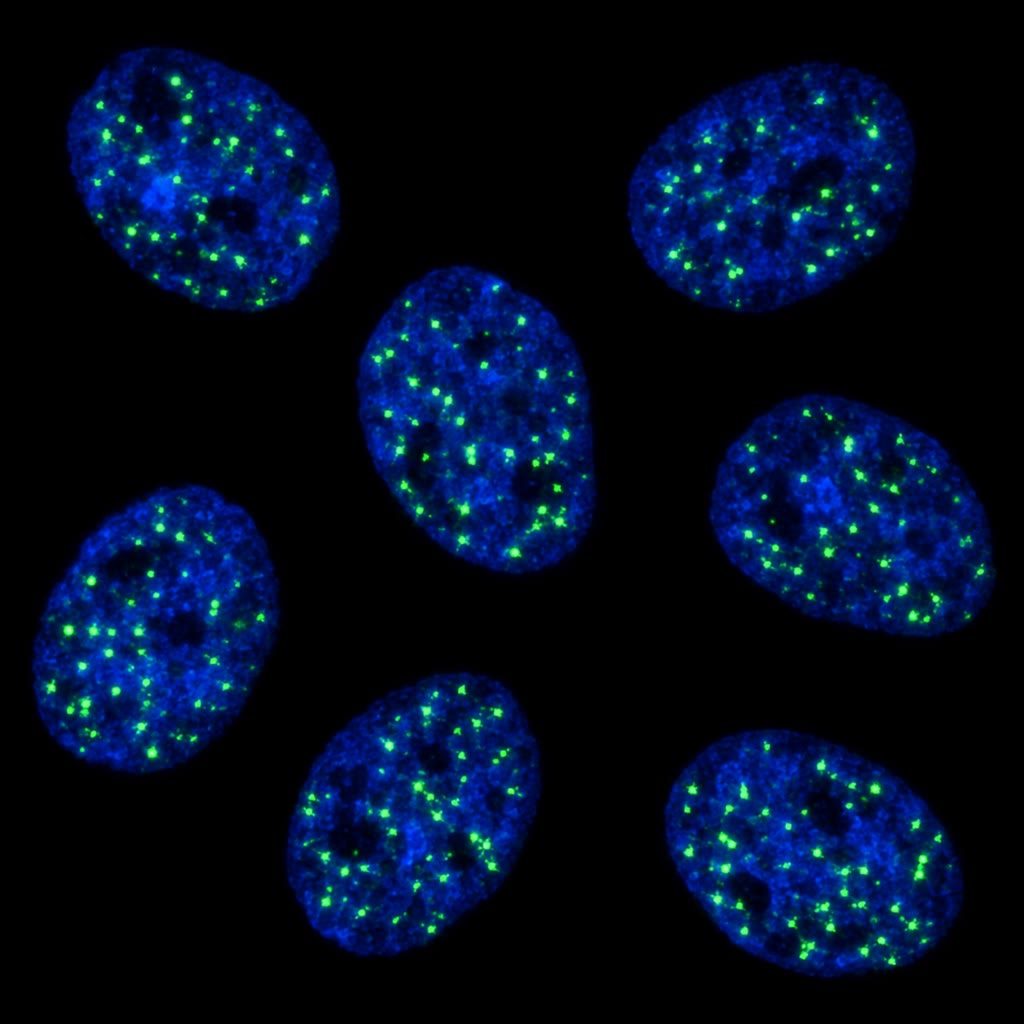
\includegraphics[width=0.4\linewidth]{images/book5/ai/b5-03-gamma-foci.jpg}

{\small Focos de $\gamma$-H2AX (verde) en núcleos (azul) una hora después
de la irradiación. Cada foco marca una \omterm{def:b3:dna-repair:lesions}{rotura de doble hebra}; contarlos
mide el daño y, en las horas siguientes, su reparación.}
\end{omfigure}

\begin{example}[Letalidad sintética: BRCA y PARP]\label{ex:b3:dna-repair:parp}
Las mujeres que heredan una copia defectuosa de \emph{BRCA1} o de
\emph{BRCA2} tienen un riesgo de cáncer de mama a lo largo de la vida del
\qtyrange{50}{80}{\%}; los tumores nacen en células que han perdido la
segunda copia y ya no pueden hacer \omterm{def:b3:dna-repair:dsb}{recombinación homóloga}. Esas células
reparan sus \omterm{def:b3:dna-repair:lesions}{roturas de doble hebra} solo por unión de extremos y acumulan
reordenamientos. Adquieren además una debilidad concreta. Las roturas de
hebra sencilla, unas \num{10000} al día, se reparan por una ruta que
necesita la enzima PARP; cuando un fármaco inhibe la PARP, las roturas de
hebra sencilla persisten hasta la fase S, donde una horquilla convierte
cada una en una \omterm{def:b3:dna-repair:lesions}{rotura de doble hebra} con un solo extremo --- reparable
solo por recombinación. Una célula normal, con un alelo \emph{\omterm{def:b3:dna-repair:dsb}{BRCA}}
bueno, se las arregla; la célula tumoral muere. Dos defectos, inocuos
cada uno por separado, son letales juntos: el fármaco mata por
\emph{letalidad sintética} y respeta las demás células del paciente.
\end{example}

\begin{proposition}[La recombinación como herramienta]\label{prop:b3:dna-repair:tools}
\index{recombinación específica de sitio}\index{Cre-lox}
Las recombinasas específicas de sitio cortan y vuelven a unir el ADN en
secuencias cortas definidas, sin búsqueda de homología ni síntesis: la
enzima Cre del fago P1 actúa sobre sitios \emph{loxP} de \qty{34}{bp}, y
la enzima Flp de la levadura sobre sitios \emph{FRT}. Dos sitios en la
misma orientación sobre una molécula escinden el ADN que hay entre ellos
en forma de círculo; en orientaciones opuestas lo invierten; y sitios
situados en dos moléculas intercambian sus flancos. Un gen flanqueado por
sitios \emph{loxP} (``flanqueado por lox'') solo se suprime en las
células donde se expresa la Cre, desde un promotor que elige quien
experimenta, o en el momento que elija si la Cre se activa con un
fármaco: así es como se estudia en el hígado adulto, o solo en una
neurona, un gen esencial para el embrión
(\cref{ch:b3:genetic-engineering}). La \omterm{def:b3:dna-repair:dsb}{recombinación homóloga} de la
propia célula es lo que toman prestado el direccionamiento génico y la
edición dirigida por CRISPR para escribir una secuencia elegida en un
lugar elegido.
\end{proposition}

\begin{remark}[Reparación y envejecimiento]\label{rem:b3:dna-repair:ageing}
Las células que no logran reparar acumulan mutaciones, entran en
senescencia o mueren; los defectos heredados de la reparación (el
síndrome de Werner, una helicasa; el síndrome de Cockayne, la reparación
acoplada a la transcripción; la ataxia telangiectasia, \omterm{def:b3:dna-repair:ddr}{ATM}) causan rasgos
de envejecimiento prematuro, y el recuento de mutaciones somáticas de los
tejidos normales sube linealmente con la edad a razón de unas decenas de
mutaciones por célula y año. Si el daño acumulado \emph{causa} el
envejecimiento ordinario, o simplemente lo acompaña, no está zanjado; que
la capacidad de reparar sea un determinante de la longevidad entre
especies --- las especies más longevas reparan más --- está bien
respaldado.
\end{remark}

\section{Ejercicios}

\begin{exercise}[$\star$]\label{exo:b3:dna-repair:1}
Clasifíquense estas lesiones como espontáneas o ambientales y nómbrese la
vía de reparación de cada una: un uracilo en el ADN; un dímero de timina;
una \omterm{def:b3:dna-repair:lesions}{8-oxoguanina}; un mal apareamiento G--T detrás de la horquilla; una
\omterm{def:b3:dna-repair:lesions}{rotura de doble hebra} en G1.
\end{exercise}

\begin{exercise}[$\star$]\label{exo:b3:dna-repair:2}
¿Por qué la \omterm{def:b3:dna-repair:excision}{reparación por escisión de nucleótidos} no necesita una enzima
específica de cada tipo de \omterm{def:b3:dna-repair:lesions}{lesión}, mientras que la \omterm{def:b3:dna-repair:excision}{reparación por
escisión de bases} necesita una \omterm{def:b3:dna-repair:excision}{glicosilasa} para cada uno?
\end{exercise}

\begin{exercise}[$\star$]\label{exo:b3:dna-repair:3}
Enúnciese el problema de la discriminación de hebra en la \omterm{prop:b3:dna-repair:fidelity}{reparación de
errores de apareamiento} y cómo lo resuelve \emph{E.~coli}. ¿Qué ocurriría
en un mutante \emph{dam}, que no metila ningún sitio GATC?
\end{exercise}

\begin{exercise}[$\star$]\label{exo:b3:dna-repair:4}
Una célula recibe \qty{2}{Gy} de rayos X. ¿Cuántas \omterm{def:b3:dna-repair:lesions}{roturas de doble hebra}
sufre, aproximadamente, y cuántos focos de $\gamma$-H2AX cabría contar
una hora después? ¿Por qué menos al cabo de seis horas?
\end{exercise}

\begin{exercise}[$\star\star$]\label{exo:b3:dna-repair:5}
Con la \cref{prop:b3:dna-repair:fidelity}, calcúlense la tasa de mutación
por par de bases y el número de mutaciones nuevas por genoma diploide y
división en (a) una célula normal, (b) una célula sin \omterm{prop:b3:dna-repair:fidelity}{reparación de
errores de apareamiento}, (c) una célula cuya polimerasa ha perdido la
exonucleasa. ¿Cuál es la mutadora más peligrosa?
\end{exercise}

\begin{exercise}[$\star\star$]\label{exo:b3:dna-repair:6}
Los sitios abásicos aparecen a razón de $10^{4}$ por célula y día y se
reparan con una semivida de \qty{15}{min}. Úsese el
\cref{thm:b3:dna-repair:load} para hallar el número estacionario de
sitios abásicos de una célula. Si un fármaco frena la reparación diez
veces, ¿cuál es el nuevo estado estacionario, y con cuántos sitios se
encontraría una horquilla que copia el genoma en \qty{8}{h}?
\end{exercise}

\begin{exercise}[$\star\star$]\label{exo:b3:dna-repair:7}
En G2 una rotura puede repararse por NHEJ (semivida \qty{30}{min}) o por
HR (semivida \qty{4}{h}), y ambas están disponibles. ¿Qué fracción de las
roturas va por HR? ¿Cuál es la semivida de las roturas? ¿Por qué es la HR
la vía que importa, de todos modos, en las horquillas de replicación
colapsadas?
\end{exercise}

\begin{exercise}[$\star\star$]\label{exo:b3:dna-repair:8}
Predíganse el comportamiento de los microsatélites, el espectro de
tumores y la sensibilidad al sol de un paciente con (a) \omterm{def:b3:dna-repair:mmr}{síndrome de
Lynch}, (b) \omterm{def:b3:dna-repair:excision}{xerodermia pigmentosa} del grupo~A, (c) la variante XP-V sin
Pol~$\eta$.
\end{exercise}

\begin{exercise}[$\star\star$]\label{exo:b3:dna-repair:9}
Dos sitios \emph{loxP} en la misma orientación flanquean el exón~3 de un
gen; la Cre se expresa desde un promotor activo solo en el hígado desde
el nacimiento. Descríbase el genotipo de las células hepáticas y de las
neuronas en el adulto, y qué ocurre si en cambio los sitios se colocan en
orientaciones opuestas.
\end{exercise}

\begin{exercise}[$\star\star\star$]\label{exo:b3:dna-repair:10}
Explíquese por qué la \omterm{prop:b3:dna-repair:sos}{respuesta SOS} enciende los genes de reparación
antes que las polimerasas propensas al error, usando las afinidades de
LexA por sus operadores, y por qué una bacteria que careciera del todo de
las polimerasas propensas al error podría estar sin embargo en desventaja
en un paciente tratado con antibióticos.
\end{exercise}

\begin{exercise}[$\star\star\star$]\label{exo:b3:dna-repair:11}
Un inhibidor de PARP mata las células tumorales deficientes en
\emph{\omterm{def:b3:dna-repair:dsb}{BRCA}} pero no las células normales del paciente. Expóngase la
cadena causal y predíganse después dos maneras en que un tumor podría
hacerse resistente al fármaco y cómo se detectaría cada una.
\end{exercise}

\begin{exercise}[$\star\star\star$]\label{exo:b3:dna-repair:12}
La conversión génica en un entrecruzamiento da tétradas $3{:}1$. Dibújese
(o descríbase) una \omterm{def:b3:dna-repair:dsb}{unión de Holliday} con un heterodúplex que abarque un
marcador, y muéstrese cómo la reparación del heterodúplex en un sentido
da $3{:}1$ y en el otro $1{:}3$, y cómo la ausencia de reparación da una
espora que es ella misma heterocigótica (una segregación posmeiótica).
¿Por qué la conversión se limita a los marcadores próximos al
entrecruzamiento?
\end{exercise}

\section{Problema: un día en la vida de un genoma}

\begin{problem}[{Problema de fin de semana --- el daño diario de una
célula humana contado, la escalera de la fidelidad multiplicada, una
dosis de sol seguida hasta la horquilla en una célula normal y en otra
deficiente en reparación, una dosis de rayos X repartida entre dos vías
de reparación y la debilidad de un tumor convertida en fármaco, hasta
llegar al número de dímeros que encuentra la horquilla, a la tasa de
mutación por base y a la fracción de roturas que repara la recombinación}]
\label{pb:b3:dna-repair:1}
Datos: una célula humana diploide tiene $6.4\times 10^{9}$ bp, de los
cuales el \qty{1.5}{\%} codifican proteína. Daño espontáneo por día:
$10^{4}$ depurinaciones, $400$ desaminaciones de citosina, $10^{4}$
roturas de hebra sencilla. Fidelidad: polimerasa $10^{-5}$, la \omterm{prop:b3:dna-repair:fidelity}{corrección
de pruebas} deja $10^{-2}$ de los errores, la \omterm{prop:b3:dna-repair:fidelity}{reparación de errores de
apareamiento} $10^{-3}$. Un baño de sol deja $10^{5}$ \omterm{def:b3:dna-repair:lesions}{dímeros de
pirimidina} por célula de piel; la reparación por escisión tiene una
semivida de \qty{2}{h} en condiciones normales y de \qty{70}{h} en la
\omterm{def:b3:dna-repair:excision}{xerodermia pigmentosa}; una horquilla llega \qty{8}{h} después; el salto
translesión de un dímero causa una mutación con probabilidad $10^{-3}$.
Los rayos X producen $35$ \omterm{def:b3:dna-repair:lesions}{roturas de doble hebra} por gray; semivida de la
NHEJ, \qty{30}{min}; semivida de la HR, \qty{4}{h}.

\medskip
\noindent\textbf{Parte I --- Días ordinarios.}
\begin{enumerate}
  \item ¿Cuántas lesiones espontáneas sufre la célula por día, y por
        año? Compárese con el tamaño del genoma.
  \item Calcúlense la tasa de mutación por par de bases y división y el
        número esperado de mutaciones nuevas por división.
  \item ¿Cuántas de ellas caen en secuencia codificante de proteína? A lo
        largo de las aproximadamente $50$ divisiones que van del cigoto a
        una célula de la piel adulta, ¿cuántas mutaciones codificantes
        lleva una célula de la piel solo por la replicación?
  \item Una célula sin \omterm{prop:b3:dna-repair:fidelity}{reparación de errores de apareamiento}: ¿tasa de
        mutación y mutaciones por división? Un microsatélite resbala una
        vez de cada $10^{4}$ divisiones sin \omterm{prop:b3:dna-repair:fidelity}{reparación de errores de
        apareamiento} y una de cada $10^{7}$ con ella. En un tumor de
        $10^{9}$ células derivadas a lo largo de $40$ divisiones,
        ¿cuántas células llevan un alelo resbalado en un microsatélite
        dado en cada caso? (Estímese con tasa $\times$ divisiones
        $\times$ células.)
  \item La \omterm{def:b3:dna-repair:lesions}{desaminación} de la citosina da uracilo; la de la
        5-metilcitosina, timina. ¿Cuál se repara, por qué medio, y cuál
        se convierte en mutación? Relaciónese con el déficit de \omterm{def:b3:chromatin-epigenetics:methylation}{CpG} del
        \cref{ch:b3:chromatin-epigenetics}.
  \item Una guanina oxidada (8-oxoG) se aparea con A durante la
        replicación. La célula tiene una \omterm{def:b3:dna-repair:excision}{glicosilasa} para la 8-oxoG
        frente a C, otra para la A frente a 8-oxoG y una hidrolasa que
        destruye el dGTP oxidado. Explíquese qué previene cada una y qué
        mutación resulta cuando fallan las tres.
\end{enumerate}

\medskip
\noindent\textbf{Parte II --- Un día al sol.}
\begin{enumerate}[resume]
  \item Calcúlense las constantes de escisión $k$ de la célula normal y
        de la XP.
  \item ¿Cuántos dímeros quedan en la horquilla en cada una?
  \item ¿Cuántas mutaciones causa el baño de sol por célula en cada caso,
        y cuántas de ellas están en secuencia codificante?
  \item A lo largo de una infancia de $500$ exposiciones de este tipo,
        ¿cuántas mutaciones codificantes por célula de la piel en cada
        caso? Compárese con la cifra de la pregunta 3, debida solo a la
        replicación.
  \item Unos $20$ genes, que suman \qty{40}{kb} de secuencia codificante,
        pueden impulsar un cáncer de piel al mutar. ¿Cuál es la
        probabilidad, por célula, de que al menos una mutación inducida
        por el sol caiga en uno de ellos, en el niño con XP? (Úsese una
        Poisson con la media adecuada.) Con $10^{9}$ células expuestas,
        ¿cuántas resultan afectadas?
  \item Explíquese por qué el problema de las células XP es de la
        horquilla y no de la \omterm{def:b3:dna-repair:lesions}{lesión} misma, y por qué los cánceres
        aparecen solo en la piel.
\end{enumerate}

\medskip
\noindent\textbf{Parte III --- Una dosis de rayos X.}
\begin{enumerate}[resume]
  \item Una dosis de \qty{2}{Gy}: ¿cuántas \omterm{def:b3:dna-repair:lesions}{roturas de doble hebra}, y
        cuántos focos de $\gamma$-H2AX al cabo de una hora si la NHEJ es
        la única vía (célula en G1)?
  \item En una célula en G2 operan las dos vías. Calcúlense las
        constantes de velocidad y la fracción de roturas que repara la
        HR.
  \item ¿Cuál es la semivida de las roturas en G2, y cuántas quedan al
        cabo de una hora?
  \item Cada suceso de NHEJ altera unos pocos pares de bases en la
        juntura. Si una juntura cae en secuencia codificante con
        probabilidad $0.015$ y la alteración estropea entonces el gen con
        probabilidad $0.7$, ¿cuántos genes estropea la dosis de
        \qty{2}{Gy} por célula en G1?
  \item Con $n$ roturas simultáneas, los extremos pueden unirse mal y dar
        una translocación. Supóngase que cada uno de los $n(n-1)/2$ pares
        de roturas se une mal con probabilidad $3\times 10^{-4}$.
        ¿Translocaciones esperadas por célula a \qty{2}{Gy}? ¿Y a
        \qty{0.2}{Gy}? ¿Por qué el riesgo escala con el cuadrado de la
        dosis mientras que el número de roturas escala linealmente?
  \item La misma dosis de \qty{2}{Gy} administrada a lo largo de
        \qty{10}{h} en lugar de en un instante: ¿cuántas roturas hay
        presentes a la vez (estado estacionario, NHEJ)? ¿Qué implica esto
        para las translocaciones y para la práctica de fraccionar la
        radioterapia?
  \item Una célula sobrevive a una dosis $D$ con probabilidad
        $e^{-D/D_{0}}$, con $D_{0} = \qty{1.5}{Gy}$ para una célula con
        la reparación intacta y \qty{0.5}{Gy} para una sin NHEJ.
        Calcúlese la supervivencia de cada una a \qty{2}{Gy} y a
        \qty{6}{Gy}, e interprétese $D_{0}$.
\end{enumerate}

\medskip
\noindent\textbf{Parte IV --- La debilidad del tumor.}
\begin{enumerate}[resume]
  \item Una célula tumoral deficiente en \emph{BRCA2} repara las roturas
        solo por NHEJ. Con la pregunta 14, ¿qué fracción de sus roturas
        de S/G2 se repara ahora de forma inexacta, que una célula normal
        habría reparado con exactitud? ¿Qué le hace esto a su genoma a lo
        largo de los años?
  \item La inhibición de PARP deja sin reparar las $10^{4}$ roturas
        diarias de hebra sencilla; el \qty{1}{\%} de ellas lo convierten
        las horquillas en \omterm{def:b3:dna-repair:lesions}{roturas de doble hebra} de un solo extremo.
        ¿Cuántas roturas así por día y célula, y por qué la NHEJ no puede
        reparar correctamente una rotura de un solo extremo?
  \item Explíquese por qué las células normales del paciente,
        heterocigóticas para \emph{BRCA2}, sobreviven al fármaco.
  \item Un tumor se hace resistente por una segunda mutación que
        restaura el marco de lectura de \emph{BRCA2}. Explíquese, y
        dígase cómo se detectaría.
  \item La quimioterapia con un agente alquilante mata las células
        tumorales a través de la \omterm{prop:b3:dna-repair:fidelity}{reparación de errores de apareamiento}:
        la enzima intenta reparar las bases alquiladas y desencadena la
        muerte celular. Predígase el efecto del fármaco sobre un tumor
        del \omterm{def:b3:dna-repair:mmr}{síndrome de Lynch}, que carece de esa reparación.
  \item Enúnciense los tres resultados: los dímeros que encuentra la
        horquilla en la célula XP (pregunta~8), la tasa normal de
        mutación por par de bases (pregunta~2) y la fracción de roturas
        de G2 que repara la HR (pregunta~14).
\end{enumerate}
\end{problem}
